 \documentclass{article}
\usepackage[utf8]{inputenc}
\usepackage[a4paper, total={7in, 10in}]{geometry}
\usepackage{braket}
\usepackage{xcolor}
\usepackage{amsmath}
\usepackage{amssymb}
\usepackage{amsfonts}
\usepackage{graphicx}
\usepackage{svg}
\usepackage{float}
\usepackage{tikz}
\usepackage[ruled,vlined]{algorithm2e}
\usepackage{multicol}
\usepackage[backend=biber,style=alphabetic,sorting=ynt]{biblatex}
\usepackage{xcolor}
%\addbibresource{sample.bib} %Import the bibliography file

\newcommand{\commentt}[1]{\textcolor{blue}{ \textbf{[COMMENT]} #1}}
\newcommand{\ctt}[1]{\commentt{#1}}
\newcommand{\prb}[1]{ \mathbf{Pr} \left[ {#1} \right]}
\newcommand{\onotation}[1]{\(\mathcal{O} \left( {#1}  \right) \)}
\newcommand{\ona}[1]{\onotation{#1}}
\newcommand{\PSI}{{\ket{\psi}}}
\newcommand{\LESn}{\ket{\psi_n}}
\newcommand{\LESa}{\ket{\phi_n}}
\newcommand{\LESs}{\frac{1}{\sqrt{n}}\sum_{i}{\ket{\left(0^{i}10^{n-i}\right)^{n}}}}
\newcommand{\Hn}{\mathcal{H}_{n}}
\newcommand{\Ep}{\frac{1}{\sqrt{2^n}}\sum^{2^n}_{x}{ \ket{xx}}}
\newcommand{\HON}{\ket{\psi_{\text{honest}}}}
\newcommand{\Lemma}{\paragraph{Lemma.}}


\setlength{\columnsep}{0.6cm}

\newcommand{\Gz}{ G_{z}^{\delta} } 

\begin{document}

\title{Quantum LTC With Positive Rate}
\author{David Ponarovsky}
\maketitle
%\begin{multicols*}{2}
\newcommand{ \Hw }{ \delta\Delta -\Delta^{\frac{1}{2}-\varepsilon}/\delta  }
	\newcommand{ \Nw }{ \Delta^{\frac{3}{2}-\varepsilon}} 
	  \newcommand{ \Gu } { \Gamma^{\cup} }
	  \newcommand{ \Guq } { \Gamma^{\cup, \square} }

    	\newcommand{ \Gsa } {\Gamma_{\square_{1}} }
	\newcommand{ \Gsb } {\Gamma_{\square_{2}} }
        \newcommand{ \Aa } { C_{A_{1}}}  
	\newcommand{ \Ab } { C_{A_{2}}}
	\newcommand{ \Ac } { C_{A_{3}}}
	\newcommand{ \Aab } { \Aa \otimes \Ab } 
	\newcommand{ \Aac } { \Aa \otimes \Ac }
	\newcommand{ \Aabc } { \Aa \otimes \Ab \otimes \Ac }
	\newcommand{ \Aabp } { \Aa^{\perp} \otimes \Ab^{\perp} } 
	\newcommand{ \Aacp } { \Aa^{\perp} \otimes \Ac^{\perp} }
	\newcommand{ \Aabcp } { \Aa^{\perp} \otimes \Ab^{\perp} \otimes \Ac^{\perp} }
	\newcommand{ \Aabpp } { \left( \Aabp \right)^\perp } 
	\newcommand{ \Aacpp } { \left( \Aacp \right)^\perp }
	\newcommand{ \Aabcpp } { \left( \Aabcp \right)^\perp }
	\newcommand{ \YY } {  y_{1}y_{2}^{\top} }
	\newcommand{ \ZZ } {  z_{1}z_{2}^{\top} } 
	\newcommand{ \TT } { \tilde{\tau} } 


  \paragraph{preamble.} preamble.  
  \begin{figure}[H]
            %\label{fig:square}
            \begin{center}
            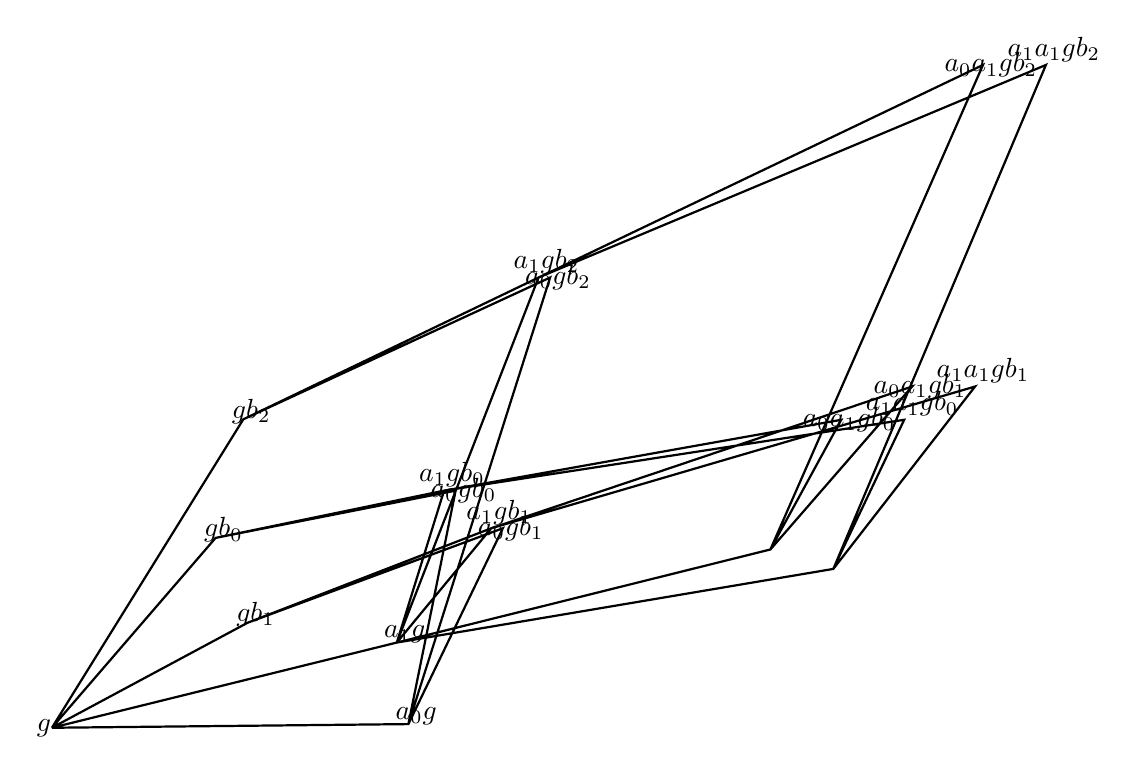
\begin{tikzpicture}
            \draw[thick](0,0)(0, 0) -- (2.0795171605737037,2.411333119673415) -- (5.12768778060503,3.011333119673415) -- (4.527687780605031,0.04664028514080889) -- (0, 0)
(0, 0) -- (2.48610403715205,1.3339314607419381) -- (5.727687780605031,2.533931460741938) -- (4.527687780605031,0.04664028514080889) -- (0, 0)
(0, 0) -- (2.431915655877046,3.917871102500838) -- (6.3276877806050305,5.717871102500838) -- (4.527687780605031,0.04664028514080889) -- (0, 0)
(0, 0) -- (2.0795171605737037,2.411333119673415) -- (4.980643044153186,3.011333119673415) -- (4.380643044153186,1.0820488771359813) -- (0, 0)
(0, 0) -- (2.48610403715205,1.3339314607419381) -- (5.580643044153186,2.533931460741938) -- (4.380643044153186,1.0820488771359813) -- (0, 0)
(0, 0) -- (2.431915655877046,3.917871102500838) -- (6.180643044153186,5.717871102500838) -- (4.380643044153186,1.0820488771359813) -- (0, 0)
(4.380643044153186, 1.0820488771359813) -- (4.980643044153186,3.011333119673415) -- (10.02505255670773,3.911333119673415) -- (9.125052556707729,2.2643026341758272) -- (4.380643044153186, 1.0820488771359813)
(4.380643044153186, 1.0820488771359813) -- (5.580643044153186,2.533931460741938) -- (10.92505255670773,4.333931460741938) -- (9.125052556707729,2.2643026341758272) -- (4.380643044153186, 1.0820488771359813)
(4.380643044153186, 1.0820488771359813) -- (6.180643044153186,5.717871102500838) -- (11.825052556707728,8.417871102500838) -- (9.125052556707729,2.2643026341758272) -- (4.380643044153186, 1.0820488771359813)
(4.380643044153186, 1.0820488771359813) -- (4.980643044153186,3.011333119673415) -- (10.824379368027538,3.911333119673415) -- (9.924379368027537,2.0174075748085016) -- (4.380643044153186, 1.0820488771359813)
(4.380643044153186, 1.0820488771359813) -- (5.580643044153186,2.533931460741938) -- (11.724379368027538,4.333931460741938) -- (9.924379368027537,2.0174075748085016) -- (4.380643044153186, 1.0820488771359813)
(4.380643044153186, 1.0820488771359813) -- (6.180643044153186,5.717871102500838) -- (12.624379368027537,8.417871102500838) -- (9.924379368027537,2.0174075748085016) -- (4.380643044153186, 1.0820488771359813)
;
\node at (5.22768778060503,3.011333119673415) {$ a_{ 0  } gb_{ 0 } $};
\node at (5.8276877806050305,2.533931460741938) {$ a_{ 0  } gb_{ 1 } $};
\node at (6.42768778060503,5.717871102500838) {$ a_{ 0  } gb_{ 2 } $};
\node at (5.080643044153185,3.2113331196734154) {$ a_{ 1  } gb_{ 0 } $};
\node at (5.680643044153186,2.733931460741938) {$ a_{ 1  } gb_{ 1 } $};
\node at (6.2806430441531855,5.917871102500838) {$ a_{ 1  } gb_{ 2 } $};
\node at (10.125052556707729,3.911333119673415) {$ a_{ 0  } a_{ 1 }gb_{ 0 } $};
\node at (11.02505255670773,4.333931460741938) {$ a_{ 0  } a_{ 1 }gb_{ 1 } $};
\node at (11.925052556707728,8.417871102500838) {$ a_{ 0  } a_{ 1 }gb_{ 2 } $};
\node at (10.924379368027537,4.111333119673415) {$ a_{ 1  } a_{ 1 }gb_{ 0 } $};
\node at (11.824379368027538,4.533931460741938) {$ a_{ 1  } a_{ 1 }gb_{ 1 } $};
\node at (12.724379368027536,8.617871102500837) {$ a_{ 1  } a_{ 1 }gb_{ 2 } $};
\node at (-0.1,0) {$ g $};
\node at (4.62768778060503,0.1466402851408089) {$ a_{ 0 }g $};
\node at (4.480643044153186,1.1820488771359814) {$ a_{ 1 }g $};
\node at (2.179517160573704,2.511333119673415) {$ gb_{ 0 } $};
\node at (2.58610403715205,1.4339314607419382) {$ gb_{ 1 } $};
\node at (2.531915655877046,4.017871102500838) {$ gb_{ 2 } $};

            \end{tikzpicture}
            \end{center}
            \caption{Square of the complex, with edges $(g,ag), (agb, gb) \in E_A,
            (g,gb), (agb, ag) \in E_B.$ \label{fig:square}
            }
            \end{figure}
 \begin{figure}[H]
            %\label{fig:square}
            \begin{center}
            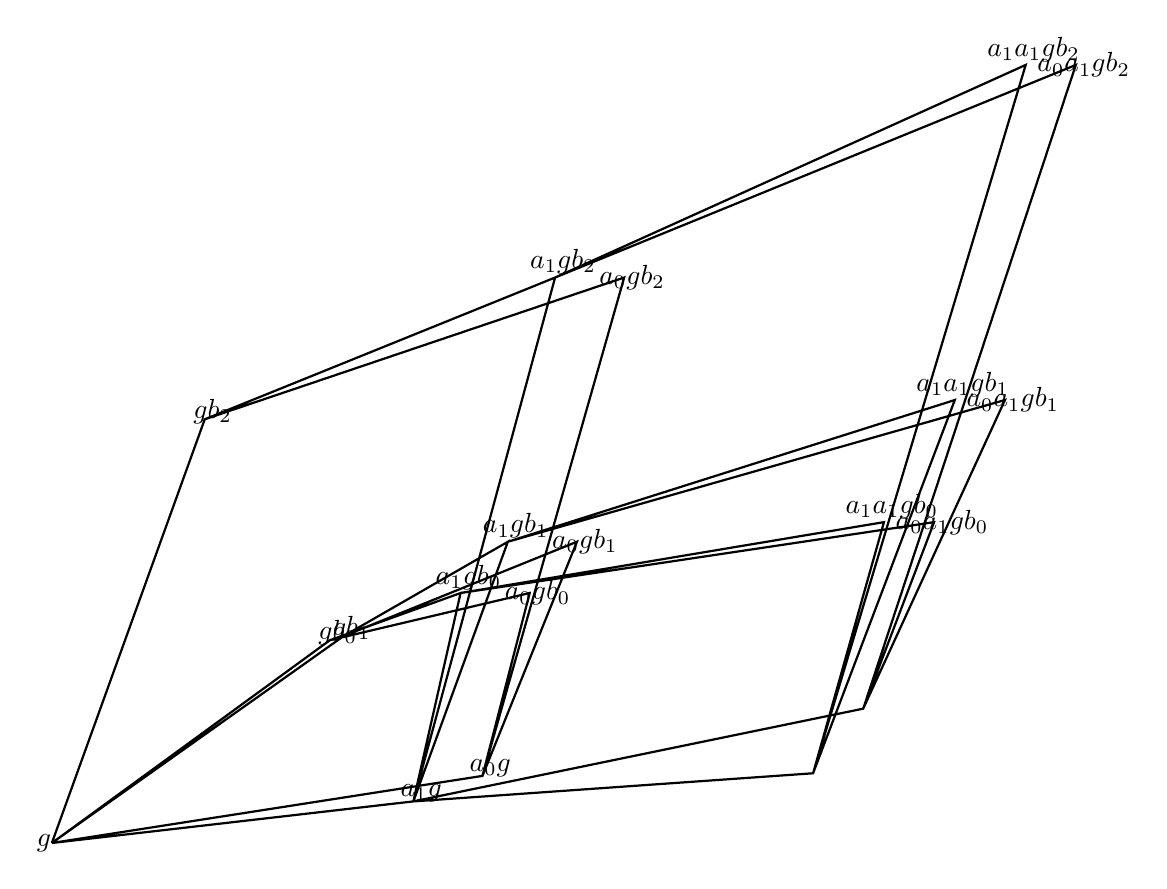
\begin{tikzpicture}
            \draw[thick](0,0)(0, 0) -- (3.529889742327744,2.5748077978352617) -- (6.068367714049943,3.174807797835262) -- (5.468367714049943,0.8520806303669085) -- (0, 0)
(0, 0) -- (3.702311476025055,2.625818649855388) -- (6.6683677140499436,3.825818649855388) -- (5.468367714049943,0.8520806303669085) -- (0, 0)
(0, 0) -- (1.9415953908618273,5.381248523807575) -- (7.268367714049943,7.181248523807575) -- (5.468367714049943,0.8520806303669085) -- (0, 0)
(0, 0) -- (3.529889742327744,2.5748077978352617) -- (5.190875696549003,3.174807797835262) -- (4.590875696549003,0.5281649429312886) -- (0, 0)
(0, 0) -- (3.702311476025055,2.625818649855388) -- (5.790875696549003,3.825818649855388) -- (4.590875696549003,0.5281649429312886) -- (0, 0)
(0, 0) -- (1.9415953908618273,5.381248523807575) -- (6.390875696549003,7.181248523807575) -- (4.590875696549003,0.5281649429312886) -- (0, 0)
(4.590875696549003, 0.5281649429312886) -- (5.190875696549003,3.174807797835262) -- (11.204164195549923,4.074807797835262) -- (10.304164195549923,1.7061825218656121) -- (4.590875696549003, 0.5281649429312886)
(4.590875696549003, 0.5281649429312886) -- (5.790875696549003,3.825818649855388) -- (12.104164195549924,5.625818649855388) -- (10.304164195549923,1.7061825218656121) -- (4.590875696549003, 0.5281649429312886)
(4.590875696549003, 0.5281649429312886) -- (6.390875696549003,7.181248523807575) -- (13.004164195549922,9.881248523807574) -- (10.304164195549923,1.7061825218656121) -- (4.590875696549003, 0.5281649429312886)
(4.590875696549003, 0.5281649429312886) -- (5.190875696549003,3.174807797835262) -- (10.567452705784222,4.074807797835262) -- (9.667452705784221,0.8855398775996648) -- (4.590875696549003, 0.5281649429312886)
(4.590875696549003, 0.5281649429312886) -- (5.790875696549003,3.825818649855388) -- (11.467452705784222,5.625818649855388) -- (9.667452705784221,0.8855398775996648) -- (4.590875696549003, 0.5281649429312886)
(4.590875696549003, 0.5281649429312886) -- (6.390875696549003,7.181248523807575) -- (12.36745270578422,9.881248523807574) -- (9.667452705784221,0.8855398775996648) -- (4.590875696549003, 0.5281649429312886)
;
\node at (6.168367714049943,3.174807797835262) {$ a_{ 0  } gb_{ 0 } $};
\node at (6.768367714049943,3.825818649855388) {$ a_{ 0  } gb_{ 1 } $};
\node at (7.368367714049943,7.181248523807575) {$ a_{ 0  } gb_{ 2 } $};
\node at (5.290875696549002,3.374807797835262) {$ a_{ 1  } gb_{ 0 } $};
\node at (5.890875696549003,4.025818649855388) {$ a_{ 1  } gb_{ 1 } $};
\node at (6.490875696549002,7.381248523807575) {$ a_{ 1  } gb_{ 2 } $};
\node at (11.304164195549923,4.074807797835262) {$ a_{ 0  } a_{ 1 }gb_{ 0 } $};
\node at (12.204164195549923,5.625818649855388) {$ a_{ 0  } a_{ 1 }gb_{ 1 } $};
\node at (13.104164195549922,9.881248523807574) {$ a_{ 0  } a_{ 1 }gb_{ 2 } $};
\node at (10.667452705784221,4.274807797835262) {$ a_{ 1  } a_{ 1 }gb_{ 0 } $};
\node at (11.567452705784222,5.825818649855388) {$ a_{ 1  } a_{ 1 }gb_{ 1 } $};
\node at (12.46745270578422,10.081248523807574) {$ a_{ 1  } a_{ 1 }gb_{ 2 } $};
\node at (-0.1,0) {$ g $};
\node at (5.568367714049943,0.9520806303669085) {$ a_{ 0 }g $};
\node at (4.690875696549003,0.6281649429312886) {$ a_{ 1 }g $};
\node at (3.629889742327744,2.674807797835262) {$ gb_{ 0 } $};
\node at (3.802311476025055,2.725818649855388) {$ gb_{ 1 } $};
\node at (2.0415953908618274,5.481248523807575) {$ gb_{ 2 } $};

            \end{tikzpicture}
            \end{center}
            \caption{Square of the complex, with edges $(g,ag), (agb, gb) \in E_A,
            (g,gb), (agb, ag) \in E_B.$ \label{fig:square}
            }
            \end{figure}
 \begin{figure}[H]
            %\label{fig:square}
            \begin{center}
            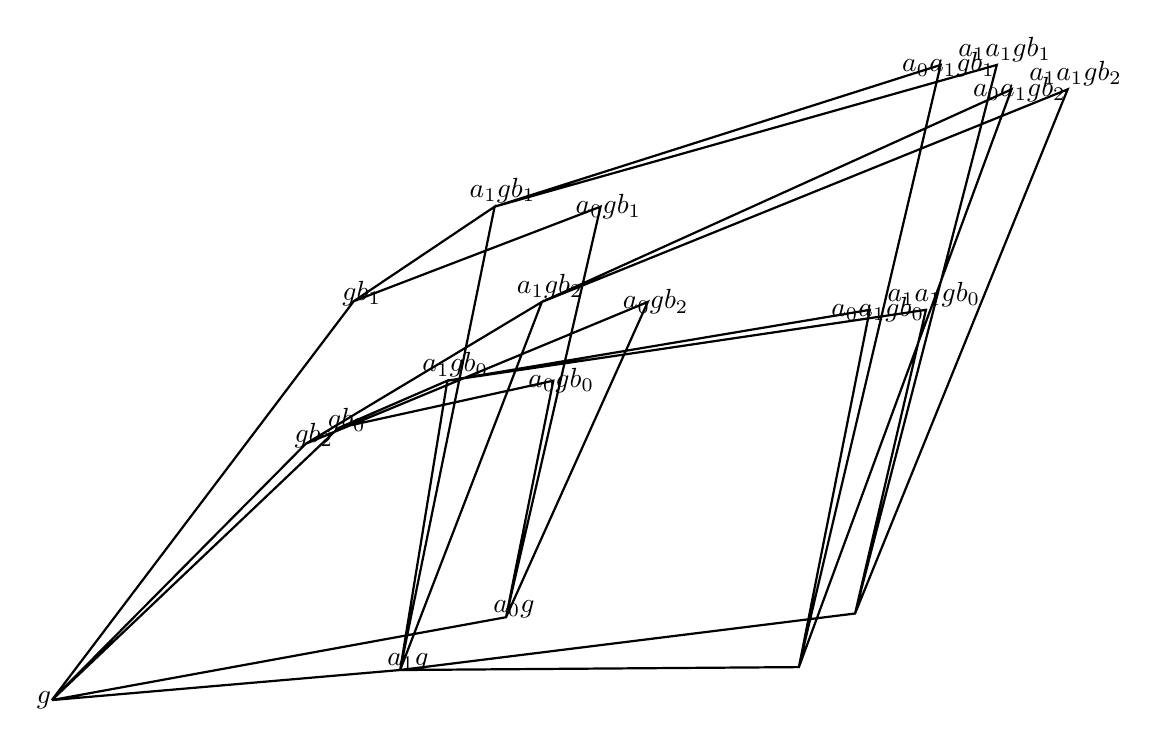
\begin{tikzpicture}
            \draw[thick](0,0)(0, 0) -- (3.6396114591143753,3.4558820574116713) -- (6.367924945592555,4.055882057411671) -- (5.767924945592555,1.0524392260813271) -- (0, 0)
(0, 0) -- (3.8345938106219233,5.0662553972720845) -- (6.967924945592555,6.266255397272085) -- (5.767924945592555,1.0524392260813271) -- (0, 0)
(0, 0) -- (3.2261313648182837,3.256073639771757) -- (7.567924945592555,5.056073639771757) -- (5.767924945592555,1.0524392260813271) -- (0, 0)
(0, 0) -- (3.6396114591143753,3.4558820574116713) -- (5.022919796608349,4.055882057411671) -- (4.422919796608349,0.38179221684495623) -- (0, 0)
(0, 0) -- (3.8345938106219233,5.0662553972720845) -- (5.6229197966083495,6.266255397272085) -- (4.422919796608349,0.38179221684495623) -- (0, 0)
(0, 0) -- (3.2261313648182837,3.256073639771757) -- (6.222919796608349,5.056073639771757) -- (4.422919796608349,0.38179221684495623) -- (0, 0)
(4.422919796608349, 0.38179221684495623) -- (5.022919796608349,4.055882057411671) -- (10.3872479402966,4.955882057411672) -- (9.4872479402966,0.4188512102855786) -- (4.422919796608349, 0.38179221684495623)
(4.422919796608349, 0.38179221684495623) -- (5.6229197966083495,6.266255397272085) -- (11.2872479402966,8.066255397272085) -- (9.4872479402966,0.4188512102855786) -- (4.422919796608349, 0.38179221684495623)
(4.422919796608349, 0.38179221684495623) -- (6.222919796608349,5.056073639771757) -- (12.1872479402966,7.756073639771757) -- (9.4872479402966,0.4188512102855786) -- (4.422919796608349, 0.38179221684495623)
(4.422919796608349, 0.38179221684495623) -- (5.022919796608349,4.055882057411671) -- (11.100643135764546,4.955882057411672) -- (10.200643135764546,1.0995080726213486) -- (4.422919796608349, 0.38179221684495623)
(4.422919796608349, 0.38179221684495623) -- (5.6229197966083495,6.266255397272085) -- (12.000643135764546,8.066255397272085) -- (10.200643135764546,1.0995080726213486) -- (4.422919796608349, 0.38179221684495623)
(4.422919796608349, 0.38179221684495623) -- (6.222919796608349,5.056073639771757) -- (12.900643135764547,7.756073639771757) -- (10.200643135764546,1.0995080726213486) -- (4.422919796608349, 0.38179221684495623)
;
\node at (6.4679249455925545,4.055882057411671) {$ a_{ 0  } gb_{ 0 } $};
\node at (7.067924945592555,6.266255397272085) {$ a_{ 0  } gb_{ 1 } $};
\node at (7.667924945592555,5.056073639771757) {$ a_{ 0  } gb_{ 2 } $};
\node at (5.122919796608349,4.255882057411672) {$ a_{ 1  } gb_{ 0 } $};
\node at (5.722919796608349,6.466255397272085) {$ a_{ 1  } gb_{ 1 } $};
\node at (6.322919796608349,5.256073639771757) {$ a_{ 1  } gb_{ 2 } $};
\node at (10.4872479402966,4.955882057411672) {$ a_{ 0  } a_{ 1 }gb_{ 0 } $};
\node at (11.3872479402966,8.066255397272085) {$ a_{ 0  } a_{ 1 }gb_{ 1 } $};
\node at (12.2872479402966,7.756073639771757) {$ a_{ 0  } a_{ 1 }gb_{ 2 } $};
\node at (11.200643135764546,5.155882057411672) {$ a_{ 1  } a_{ 1 }gb_{ 0 } $};
\node at (12.100643135764546,8.266255397272085) {$ a_{ 1  } a_{ 1 }gb_{ 1 } $};
\node at (13.000643135764546,7.956073639771757) {$ a_{ 1  } a_{ 1 }gb_{ 2 } $};
\node at (-0.1,0) {$ g $};
\node at (5.867924945592555,1.1524392260813272) {$ a_{ 0 }g $};
\node at (4.522919796608349,0.4817922168449562) {$ a_{ 1 }g $};
\node at (3.7396114591143754,3.5558820574116714) {$ gb_{ 0 } $};
\node at (3.9345938106219234,5.166255397272084) {$ gb_{ 1 } $};
\node at (3.3261313648182838,3.356073639771757) {$ gb_{ 2 } $};

            \end{tikzpicture}
            \end{center}
            \caption{Square of the complex, with edges $(g,ag), (agb, gb) \in E_A,
            (g,gb), (agb, ag) \in E_B.$ \label{fig:square}
            }
            \end{figure}
 \begin{figure}[H]
            %\label{fig:square}
            \begin{center}
            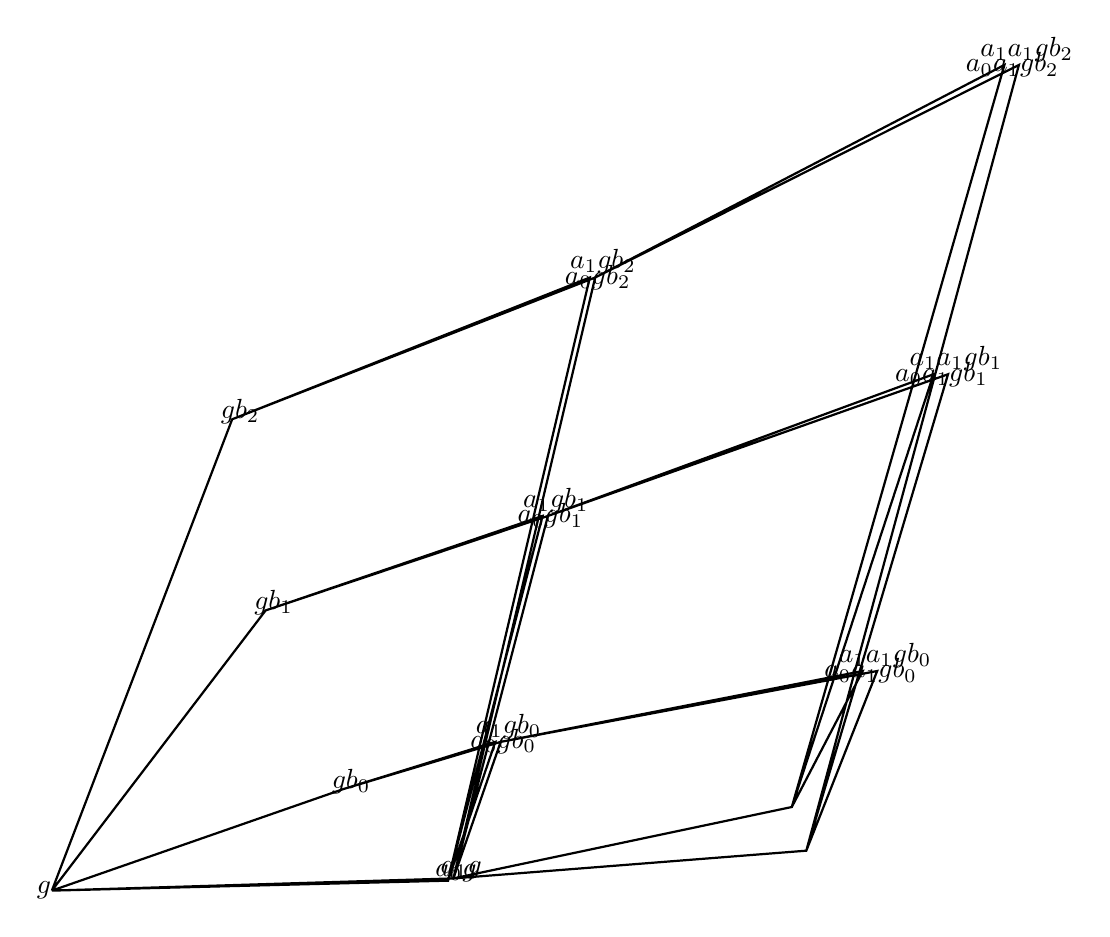
\begin{tikzpicture}
            \draw[thick](0,0)(0, 0) -- (3.6994269858984827,1.288738348949305) -- (5.631600576759389,1.888738348949305) -- (5.03160057675939,0.12627015480875062) -- (0, 0)
(0, 0) -- (2.714645993603899,3.5579125766659354) -- (6.23160057675939,4.757912576665936) -- (5.03160057675939,0.12627015480875062) -- (0, 0)
(0, 0) -- (2.289950433154898,5.985964509032648) -- (6.8316005767593895,7.785964509032648) -- (5.03160057675939,0.12627015480875062) -- (0, 0)
(0, 0) -- (3.6994269858984827,1.288738348949305) -- (5.699553942007855,1.888738348949305) -- (5.099553942007855,0.15488289691761925) -- (0, 0)
(0, 0) -- (2.714645993603899,3.5579125766659354) -- (6.299553942007855,4.757912576665936) -- (5.099553942007855,0.15488289691761925) -- (0, 0)
(0, 0) -- (2.289950433154898,5.985964509032648) -- (6.899553942007855,7.785964509032648) -- (5.099553942007855,0.15488289691761925) -- (0, 0)
(5.099553942007855, 0.15488289691761925) -- (5.699553942007855,1.888738348949305) -- (10.297201907231647,2.788738348949305) -- (9.397201907231647,1.061784392125702) -- (5.099553942007855, 0.15488289691761925)
(5.099553942007855, 0.15488289691761925) -- (6.299553942007855,4.757912576665936) -- (11.197201907231648,6.557912576665935) -- (9.397201907231647,1.061784392125702) -- (5.099553942007855, 0.15488289691761925)
(5.099553942007855, 0.15488289691761925) -- (6.899553942007855,7.785964509032648) -- (12.097201907231646,10.485964509032648) -- (9.397201907231647,1.061784392125702) -- (5.099553942007855, 0.15488289691761925)
(5.099553942007855, 0.15488289691761925) -- (5.699553942007855,1.888738348949305) -- (10.481247042234655,2.788738348949305) -- (9.581247042234654,0.5070379797628226) -- (5.099553942007855, 0.15488289691761925)
(5.099553942007855, 0.15488289691761925) -- (6.299553942007855,4.757912576665936) -- (11.381247042234655,6.557912576665935) -- (9.581247042234654,0.5070379797628226) -- (5.099553942007855, 0.15488289691761925)
(5.099553942007855, 0.15488289691761925) -- (6.899553942007855,7.785964509032648) -- (12.281247042234654,10.485964509032648) -- (9.581247042234654,0.5070379797628226) -- (5.099553942007855, 0.15488289691761925)
;
\node at (5.731600576759389,1.888738348949305) {$ a_{ 0  } gb_{ 0 } $};
\node at (6.3316005767593895,4.757912576665936) {$ a_{ 0  } gb_{ 1 } $};
\node at (6.931600576759389,7.785964509032648) {$ a_{ 0  } gb_{ 2 } $};
\node at (5.799553942007854,2.088738348949305) {$ a_{ 1  } gb_{ 0 } $};
\node at (6.399553942007855,4.957912576665936) {$ a_{ 1  } gb_{ 1 } $};
\node at (6.9995539420078545,7.985964509032648) {$ a_{ 1  } gb_{ 2 } $};
\node at (10.397201907231647,2.788738348949305) {$ a_{ 0  } a_{ 1 }gb_{ 0 } $};
\node at (11.297201907231647,6.557912576665935) {$ a_{ 0  } a_{ 1 }gb_{ 1 } $};
\node at (12.197201907231646,10.485964509032648) {$ a_{ 0  } a_{ 1 }gb_{ 2 } $};
\node at (10.581247042234654,2.988738348949305) {$ a_{ 1  } a_{ 1 }gb_{ 0 } $};
\node at (11.481247042234655,6.757912576665936) {$ a_{ 1  } a_{ 1 }gb_{ 1 } $};
\node at (12.381247042234653,10.685964509032647) {$ a_{ 1  } a_{ 1 }gb_{ 2 } $};
\node at (-0.1,0) {$ g $};
\node at (5.131600576759389,0.22627015480875062) {$ a_{ 0 }g $};
\node at (5.199553942007855,0.25488289691761923) {$ a_{ 1 }g $};
\node at (3.799426985898483,1.388738348949305) {$ gb_{ 0 } $};
\node at (2.814645993603899,3.6579125766659355) {$ gb_{ 1 } $};
\node at (2.389950433154898,6.085964509032648) {$ gb_{ 2 } $};

            \end{tikzpicture}
            \end{center}
            \caption{Square of the complex, with edges $(g,ag), (agb, gb) \in E_A,
            (g,gb), (agb, ag) \in E_B.$ \label{fig:square}
            }
            \end{figure}
 
%\end{multicols*}
  % \printbibliography 
\end{document}

 